\chapter{Introdução}
\label{chap:intro}

As Tecnologias de Informação e Comunicação (TICs) conquistam mais espaço e se consolida no cotidiano das pessoas \cite{Sales2020}. Essa interação entre seres humanos e as TICs abrange diversos tipos de perfis de usuários e de contexto de uso, assim é exigido do profissional, que desenvolvem essas tecnologias, certas habilidades. A habilidade de criar esses sistemas, envolve o conhecimento de técnicas, ferramentas e métodos que englobam tanto a Engenharia de Software (ES) quanto a área de Interação Humano-Computador (IHC) \cite[p. 2]{barbosa_silva}.  

Na Engenharia de Software, o campo de IHC preocupa-se em definir como serão as interações entre as ações humanas e os sistemas computacionais, elaborando interfaces para que isso seja possível \cite{queiroz, sommariva} \cite[p. 89,90]{acm_curricula}. O ensino de IHC nos cursos de graduação e pós-graduação na área de Tecnologia da Informação (TI), como é o caso da Engenharia de Software, possui esse objetivo, propiciar a formação de profissionais qualificados capazes de desenvolver interfaces para sistemas computacionais com qualidade, direcionados a atender de forma satisfatória às necessidade e expectativas do usuário \cite[p. 89,  90]{acm_curricula} \cite[p. 7-14]{barbosa_silva}. No entanto os princípios oriundos do campo de IHC podem não ser tão bem aderidos pelos profissionais que desenvolvem software, que acabam por tratar esses conceitos como secundários. Isso se deve a falta de compreensão desses profissionais, que focam mais na parte interna dos sistemas \cite{sommariva}.

O meio acadêmico tem investido no uso de novas abordagens e tecnologias como recurso complementar no processo de ensino-aprendizagem, auxiliando no desenvolvimento de atividades pedagógicas inovadoras e colaborativas em diversas áreas \cite{battistella, brito}, incluindo em IHC \cite{Sales2020,Sales2020UsoTDS}. Os jogos sérios fazem parte dessas abordagens que vêm se tornando cada vez mais populares na educação em computação, pois podem aumentar a eficácia e o engajamento da aprendizagem \cite{battistella, brito, queiroz}.

Esse cenário motivou a criação de jogos educacionais com o objetivo de auxiliar o ensino e aprendizagem de IHC voltado para cursos de graduação e pós-graduação na área de Ciência da Computação. Diversas propostas de jogos para o ensino-aprendizagem de IHC já existem, seja com o intuito de introduzir conceitos iniciais, reforçá-los ou desenvolver habilidades mais práticas \cite{darin}. Dentre estes pode-se citar o UsabilityGame \cite{sommariva}, UsabiliCity \cite{ferreira2014a,ferreira2014b} e MACteaching \cite{brito,queiroz} como também jogos não-digitais como Desafio Goople \cite{darin}, G4H \cite{juca2017} e o G4NHE \cite{deSousa2019} .

Este trabalho visa o desenvolvimento de um jogo que auxilie o processo de ensino e aprendizagem em IHC em curso de graduação e pós-graduação, porém com um conteúdo diferente dos jogos já existentes. O conteúdo disciplinar o qual este jogo trata é a técnica de \textit{Personas}. Conforme é citado por \cite[p. 176]{barbosa_silva}, com base nos autores \citeonline{cooper99, pruitt, cooper07}, \textit{"uma persona é um personagem fictício, arquétipo hipotético de um grupo de usuários reais, criada para descrever um usuário típico"}. 

Em outras palavras, embora fictícia, uma \textit{persona} é definida com um rigor de detalhes de forma que represente bem o público-alvo de usuários reais, para o qual a interface deve ser direcionada  \cite[p. 177]{barbosa_silva}. Sendo assim, essa técnica é uma ferramenta poderosa para a elaboração do design, pois uma vez que ele atenda os objetivos das personas elencadas, o design da interface estará satisfazendo seus usuários reais \cite[p. 77]{cooper99}.

Para um engenheiro de software ter o conhecimento de tal técnica se faz necessário em situações nas quais o público-alvo do sistema engloba muitas pessoas ou que é custosa a presença frequente do usuário durante as etapas do projeto. Desta forma torna-se difícil a validação constante do design, o que pode acarretar num produto que não atenda os objetivos e necessidades do cliente \cite[p. 176]{barbosa_silva}.

Num cenário de trabalho remoto, onde existe essa dificuldade de interação com o usuário, a importância do conhecimento desta técnica para o profissional de desenvolvimento de software justifica a escolha do tema do jogo. Neste trabalho é apresentado o PersonaDesignGame, um jogo educacional sobre personas. Ele é um jogo do gênero de perguntas e respostas, onde o jogador progride ao responder corretamente às questões. Ao longo das fases o jogador recebe recompensas, que irão compor algumas personas e ao final, o jogador terá exemplos de personas. Na seção a seguir são detalhados os objetivos geral e específicos deste trabalho.

\section{Objetivos}

\subsection{Objetivo Geral}

O objetivo geral deste trabalho é desenvolver um jogo digital que auxilie o processo de ensino-aprendizagem dos conceitos sobre \textit{personas} em IHC.

\subsection{Objetivo Específico}
\begin{itemize}
    \item \textbf{OE01} - Desenvolver conhecimento sobre os conceitos principais envolvidos neste trabalho;
    \item \textbf{OE02} - Utilizar personas que representem os jogadores-alvo durante o processo de desenvolvimento;
    \item \textbf{OE03} - Aplicar alguns conceitos fundamentais da Engenharia de Software, no processo de design e desenvolvimento de um jogo digital; e    
    \item \textbf{OE04} - Desenvolver o jogo digital para apoio ao ensino e aprendizado de personas;
    \item \textcolor{blue}{\textbf{OE05} - Aplicar conceitos de DevOps para a configuração do ambiente de desenvolvimento de um jogo digital.}
\end{itemize}

\section{Plano de Trabalho}

Primeiramente foi realizado o planejamento identificando os requisitos necessários para a realização do projeto, mapeando as atividades a serem realizadas e construindo um cronograma \cite[p. 74]{Pressman_2000}. Foi tomado por base a própria dinâmica do desenvolvimento do Trabalho de Conclusão de Curso, onde este projeto é dividido em duas fases: TCC1 e TCC2. Na Figura \ref{Fig:eap.png}, são apresentadas as fases e suas respectivas atividades em forma de uma Estrutura Analítica de Projeto \cite[p. 112]{pmbok}. %ES pg 74

\begin{figure}[htbp]
	\centering
		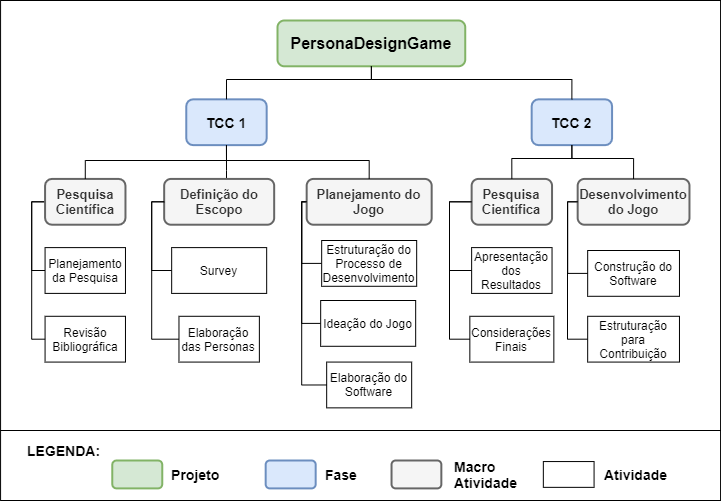
\includegraphics[keepaspectratio=true,scale=0.60]{figuras/eap.png}
	\caption{Estrutura Analítica do Projeto - Próprio Autor}
	\label{Fig:eap.png}
\end{figure}

As macro atividades apresentadas na EAP tem relação com o objetivo deste trabalho. Elas são subdivididas outras vez, evidenciando atividades mais específicas que têm propósito de atingir os seus objetivos específicos. Abaixo é relatada a relação entre atividades e objetivos. 

Na fase do TCC 1:

\begin{itemize}
    \item A macro atividade Pesquisa Científica é composta pelas atividades de Planejamento da Pesquisa e Revisão Bibliográfica tendo como finalidade alcançar o OE01;
    \item A macro atividade Definição do Escopo é formada pelas atividades do Survey e Elaboração das Personas com foco em alcançar o OE02; e
    \item A macro atividade Planejamento do Jogo é composta pelas atividades de Estruturação do Processo de Desenvolvimento, Ideação do Jogo e Elaboração do Software possuindo como objetivo o OE02, o OE03 e o OE04.
\end{itemize}

Na fase do TCC 2:

\begin{itemize}
    \item A macro atividade Pesquisa Científica é composta pelas atividades de Apresentação dos Resultados e Considerações Finais tendo como objetivo o OE01; e
    \item A macro atividade Desenvolvimento do Jogo é composta pelas atividades de Construção do Software e Estruturação para Contribuição possuindo como objetivo o OE02, OE03 e OE04.
\end{itemize}

Essas atividades são abordadas ao longo do projeto por meio de passos, etapas e tarefas. Estas estão apresentadas no Capítulo \ref{chap:Metodo}, estando elas organizadas num processo metodológico a fim de serem alcançados os objetivos deste estudo. Segue apresentado na Figura \ref{Fig:cronograma.png} o cronograma destas atividades ao longo das fases de entrega, TCC 1 e TCC 2.

\newpage
\begin{figure}[htbp]
	\centering
		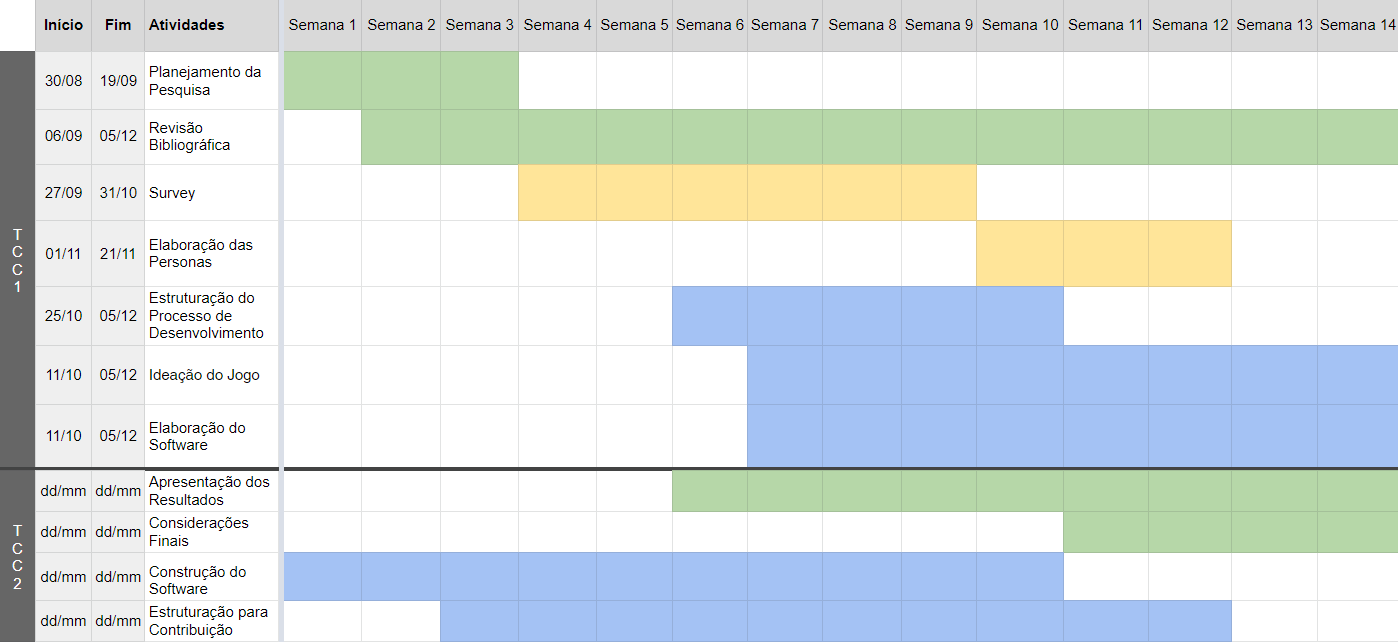
\includegraphics[keepaspectratio=true,scale=0.42]{figuras/cronograma.png}
	\caption{Cronograma de Trabalho - Fonte: Próprio Autor}
	\label{Fig:cronograma.png}
\end{figure}

\section{Estrutura do Trabalho}

Este trabalho está estruturado, até o momento, em quatro capítulos. O presente capítulo mostra uma visão geral dos conceitos que contextualizam este trabalho. Além disso é apresentado seu objetivo, o plano de trabalho e sua estrutura organizacional.

O Capítulo \ref{chap:Metodo}, apresenta a estrutura do processo metodológico utilizado neste trabalho. Nele é relatado a metodologia usada da revisão da bibliográfica até o desenvolvimento do jogo.  

O Capítulo \ref{chap:ref}, apresenta os principais conceitos que envolvem este trabalho e como eles se relacionam. Neste capítulo está descrito uma base sobre IHC, Personas e Jogos.

O Capítulo \ref{chap:des}, apresenta o progresso do desenvolvimento do projeto. Neste primeiro momento são relatados resultados parciais do design técnico e de ideação do jogo.

%O capítulo Apresentação dos Resultados...

%O capítulo Considerações Finais ...